\documentclass[a4paper]{article}
% mathematische symbolen
\usepackage{geometry}
\geometry{verbose,a4paper,tmargin=2.5cm,bmargin=2.5cm,lmargin=2.5cm,rmargin=2.5cm}
\usepackage[dutch]{babel}
\usepackage{hyperref}
\usepackage{graphicx}
\usepackage{tabularx}
\usepackage{booktabs}
\usepackage{amssymb}
\usepackage{amsmath,amsthm}
\usepackage{latexsym}
\usepackage{amsfonts}
\usepackage{qtree}
\usepackage{mathrsfs}
% the following to packages are for nice looking algorithms
\usepackage[]{algorithm} 	% use [section] to number algorithms according to their section
\usepackage{algpseudocode}
% Package for automata visualization
\usepackage{tikz}
\usetikzlibrary{automata,positioning}
\title{Berekenbaarheidstheorie (TI2320), Opgave 2} 
\author{Elgar de Groot\\ 
4091108
\and Ewout den Heijer\\
4025695}
\date{}
\begin{document}
\maketitle %produceert de daadwerkelijke titelinformatie

\section*{Opgave}
Construeer een Turing-machine met invoer-alfabet $\sum = \{1, \#\}$ die de taal L gedefinieerd door $L=\{1^x\#1^y | x$ mod $2 = y$ mod $3\}$
accepteert.

\section*{Oplossing}

We zullen aannemen dat de invoer als volgt op de tape staat (bijvoorbeeld voor $x=2$ en $y=3$):
\begin{align*}
11\#111
\end{align*}
Bovendien nemen we aan dat de lees/schrijfkop van de TM, van links naar rechts gezien, op het eerste symbool van de invoer staat.

\subsection*{Globale opzet van de TM}
We kiezen voor de Turingmachine het volgende alfabet: 
\begin{align*}
\sum = \{1,\#,a,b,c\}
\end{align*}
De werking van de TM is als volgt. De TM accepteerd een woord als het 2 reeksen 1-en heeft, gescheiden door een \#, waarbij de rest na deling door 2 van de eerste reeks gelijk is aan de rest na deling door 3 van de tweede reeks.

\subsection*{Implementatie-beschrijving}
De implementatie-beschrijving van het algoritme luidt als volgt:
\begin{enumerate}
\item Lees het symbool onder de kop. Als het een hekje is, ga dan naar stap 6. Is het een 1, ga dan door.
\item Ga een stap naar links en lees het symbool onder de kop.
\item Is het het einde van de tape of een b, ga dan weer naar rechts en herschrijf naar een a. Is het een a, ga dan weer naar rechts en herschrijf naar een b.
\item Ga een stap naar rechts.
\item Herhaal stap 1-5.
\item Ga helemaal naar rechts tot het laatste symbool.
\item Lees het symbool onder de kop. Is het een hekje, ga dan naar stap 12. Is het een 1 ga dan door.
\item Ga een stap naar rechts en lees het symbool onder de kop.
\item Is het het einde van de tape of een c, ga dan weer naar links en herschrijf naar een a. Is het een b, ga dan weer naar links en herschrijf naar een c. Is het een a, ga dan weer naar links en herschrijf naar een c.
\item Ga een stap naar links.
\item Herhaal stap 6-11.
\item Ga een stap naar links en lees het symbool onder de kop. 
\item Is het een b of het eind van de tape, ga dan twee stappen naar rechts en lees het symbool onder de kop. Als dit een c is of het eind van de tape, accepteer het woord.
\item Is het een a, ga dan 2 stappen naar rechts en lees het symbool onder de kop. Als dit ook een a is, accepteer dan het woord.
\end{enumerate}
\subsection*{Toestandsdiagram}
\begin{center}
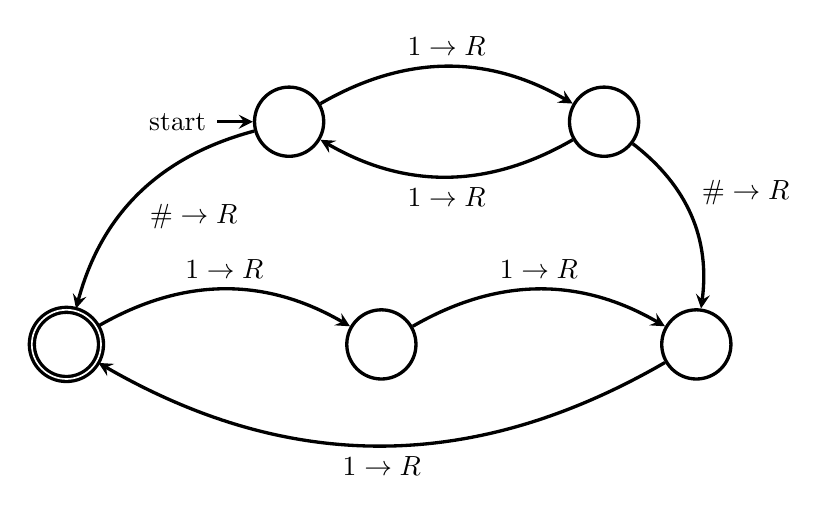
\begin{tikzpicture}[%
       >=stealth,
       node distance=4cm,
       very thick,
       on grid,
       auto
     ]
     \node[initial,state]		(0)       				{};
     \node[state] 			  	(1) [right of=0]			{};
     \node[state,accepting]	  	(2) [below left of=0]	{};
     \node[state] 			  	(3) [right of=2]			{};
     \node[state]			  	(4) [right of=3]			{};
     
     \path[->] (0) edge[bend left]		node {$1\rightarrow R$} 			(1);
     \path[->] (1) edge[bend left]		node {$1\rightarrow R$} 			(0);
     \path[->] (0) edge[bend right]		node {$\#\rightarrow R$}			(2);
     \path[->] (1) edge[bend left]		node {$\#\rightarrow R$}		 	(4);
     \path[->] (2) edge[bend left]		node {$1\rightarrow R$} 			(3);
     \path[->] (3) edge[bend left]		node {$1\rightarrow R$} 			(4);
     \path[->] (4) edge[bend left]		node {$1\rightarrow R$} 			(2);
\end{tikzpicture}
\end{center}

\end{document}